\documentclass[11pt,a4paper]{article}

% --- Packages ---
\usepackage[utf8]{inputenc}
\usepackage[margin=0.75in]{geometry}
\usepackage{amsmath,amssymb,amsfonts}
\usepackage{booktabs,multirow,array,colortbl}
\usepackage[table,dvipsnames]{xcolor}
\usepackage{tikz}
\usetikzlibrary{shapes.geometric, arrows.meta, positioning, calc, shadows, fit, backgrounds}
\usepackage[most]{tcolorbox}
\usepackage{fancyhdr}
\usepackage{hyperref}
\usepackage{enumitem}

% --- Color Palette ---
\definecolor{primaryblue}{RGB}{24, 43, 73}
\definecolor{secondaryblue}{RGB}{41, 128, 185}
\definecolor{accentteal}{RGB}{0, 150, 136}
\definecolor{lightgrey}{RGB}{245, 247, 250}
\definecolor{darkgrey}{RGB}{50, 50, 50}
\definecolor{tableheader}{RGB}{220, 235, 252}
\definecolor{tablerowalt}{RGB}{242, 247, 255}

% --- Hyperref Setup ---
\hypersetup{
    colorlinks=true,
    linkcolor=primaryblue,
    citecolor=secondaryblue,
    urlcolor=accentteal,
    pdftitle={Basic Computer Registers: Theory, Architecture, and Execution Trace},
    pdfauthor={Computer Organization and Architecture}
}

% --- Header and Footer ---
\pagestyle{fancy}
\fancyhf{}
\setlength{\headheight}{14pt}
\rhead{\textcolor{primaryblue}{\small\textbf{Basic Computer Registers Theory}}}
\lhead{\textcolor{primaryblue}{\small\textbf{Computer Organization \& Architecture}}}
\rfoot{\thepage}
\lfoot{\textcolor{darkgrey}{\small Confidential / Educational Reference}}
\renewcommand{\headrulewidth}{0.8pt}
\renewcommand{\footrulewidth}{0.4pt}

% --- Custom Box Styling ---
\newtcolorbox{summarybox}[1]{
    colback=lightgrey,
    colframe=primaryblue,
    fonttitle=\bfseries\color{white},
    title=#1,
    arc=3mm,
    boxrule=1pt,
    left=10pt,
    right=10pt,
    top=8pt,
    bottom=8pt
}

\newtcolorbox{registerbox}[2]{
    colback=tablerowalt,
    colframe=secondaryblue,
    fonttitle=\bfseries\color{white},
    title={#1 (\texttt{#2})},
    arc=2mm,
    boxrule=0.8pt,
    left=8pt,
    right=8pt,
    top=6pt,
    bottom=6pt
}

% --- Document Starts ---
\begin{document}

% --- Title Block ---
\begin{center}
    {\LARGE \textbf{\textcolor{primaryblue}{Fundamental Registers in Basic Computer Architecture}}}\\[0.3cm]
    {\large \textbf{\textcolor{secondaryblue}{Comprehensive Theory, Bus System Interconnect, Tabled Execution Trace, and Circuit Diagrams}}}\\[0.2cm]
    \hrule height 1.5pt
    \vspace{0.3cm}
    {\small \textbf{Course:} Computer Organization and Architecture \quad|\quad \textbf{Topic:} Basic Computer Register Set \& Common Bus System}
    \vspace{0.3cm}
\end{center}

\begin{summarybox}{Executive Summary \& Architectural Overview}
In a basic computer system (such as the classic Mano Machine model), the Central Processing Unit (CPU) relies on a dedicated set of internal hardware registers. Registers are high-speed storage elements constructed from flip-flops that store binary information during program execution. Memory contains instructions and data, but processor registers hold immediate operational operands, instruction codes, memory pointers, and I/O buffer bytes. 

The architecture evaluated here comprises an overall memory unit of $4096 \times 16$ bits ($4\text{K}$ words of 16 bits each). Consequently, memory addresses require $\mathbf{12\text{ bits}}$ ($2^{12} = 4096$), while data words require $\mathbf{16\text{ bits}}$. Input and output character transfers utilize $\mathbf{8\text{ bits}}$ (ASCII).
\end{summarybox}

\vspace{0.2cm}

% ==========================================
% SECTION 1: DETAILED REGISTER SPECIFICATIONS
% ==========================================
\section{\textcolor{primaryblue}{Detailed Theoretical Analysis of Registers}}

The basic computer contains eight primary hardware registers, each serving a specialized role in the fetch-decode-execute instruction cycle and input/output subsystem.

\begin{registerbox}{Address Register}{AR}
\textbf{Bit Width:} 12 Bits \quad|\quad \textbf{Bus Selection Code:} $(001)_2$ \quad|\quad \textbf{Directly Memory Connected: Yes}\\[0.1cm]
The Address Register ($\text{AR}$) holds the 12-bit address of the memory location currently being accessed for a read or write operation. Because memory capacity is 4096 words, $\text{AR}$ is 12 bits wide ($2^{12} = 4096$). 
\begin{itemize}[noitemsep,topsep=2pt]
    \item \textbf{Function:} Provides physical address signals directly to the address lines of the RAM module.
    \item \textbf{Control Inputs:} Load ($\text{LD}$), Increment ($\text{INR}$), Clear ($\text{CLR}$), Clock ($\text{CLK}$).
    \item \textbf{Microoperations:} $\text{AR} \leftarrow \text{PC}$ (during instruction fetch), $\text{AR} \leftarrow \text{IR}(0-11)$ (during address decoding), $\text{AR} \leftarrow \text{AR} + 1$.
\end{itemize}
\end{registerbox}

\vspace{0.15cm}

\begin{registerbox}{Program Counter}{PC}
\textbf{Bit Width:} 12 Bits \quad|\quad \textbf{Bus Selection Code:} $(010)_2$ \quad|\quad \textbf{Role:} Instruction Sequence Control\\[0.1cm]
The Program Counter ($\text{PC}$) contains the 12-bit address of the next instruction to be fetched from memory.
\begin{itemize}[noitemsep,topsep=2pt]
    \item \textbf{Function:} Maintains the sequential flow of program execution. After fetching an instruction into the Instruction Register, $\text{PC}$ is automatically incremented by 1.
    \item \textbf{Branching Logic:} During jump ($\text{JMP}$) or branch instructions, the target address from $\text{AR}$ or $\text{IR}$ is loaded into $\text{PC}$, altering sequential execution.
    \item \textbf{Microoperations:} $\text{PC} \leftarrow \text{PC} + 1$ (Fetch phase step $T_1$), $\text{PC} \leftarrow \text{AR}$ (Branching step).
\end{itemize}
\end{registerbox}

\vspace{0.15cm}

\begin{registerbox}{Data Register}{DR}
\textbf{Bit Width:} 16 Bits \quad|\quad \textbf{Bus Selection Code:} $(011)_2$ \quad|\quad \textbf{Role:} Memory Operand Buffer\\[0.1cm]
The Data Register ($\text{DR}$) holds the 16-bit operand read from memory or the operand ready to be written to memory.
\begin{itemize}[noitemsep,topsep=2pt]
    \item \textbf{Function:} Serves as a buffer between high-speed CPU registers/ALU and memory data lines. During arithmetic/logic execution (e.g., \texttt{ADD}, \texttt{AND}), $\text{DR}$ feeds the second operand directly into the Arithmetic Logic Unit (ALU).
    \item \textbf{Microoperations:} $\text{DR} \leftarrow M[\text{AR}]$ (Memory Read), $\text{DR} \leftarrow \text{AC}$ (Memory Write prep), $\text{DR} \leftarrow \text{DR} + 1$.
\end{itemize}
\end{registerbox}

\vspace{0.15cm}

\begin{registerbox}{Accumulator}{AC}
\textbf{Bit Width:} 16 Bits \quad|\quad \textbf{Bus Selection Code:} $(100)_2$ \quad|\quad \textbf{Role:} Primary Working \& ALU Register\\[0.1cm]
The Accumulator ($\text{AC}$) is the central general-purpose processing register. It stores the primary operand before an operation and receives the final result produced by the ALU.
\begin{itemize}[noitemsep,topsep=2pt]
    \item \textbf{Extended Bit ($E$):} $\text{AC}$ is associated with a 1-bit overflow/carry flip-flop ($E$).
    \item \textbf{Microoperations:} $\text{AC} \leftarrow \text{AC} + \text{DR}$ (Addition), $\text{AC} \leftarrow \text{AC} \wedge \text{DR}$ (Logical AND), $\text{AC} \leftarrow \overline{\text{AC}}$ (Complement), $\text{AC} \leftarrow 0$ (Clear), $\text{AC} \leftarrow \text{shr } \text{AC}$ (Shift Right), $\text{AC} \leftarrow \text{INPR}(0-7)$ (Input transfer).
\end{itemize}
\end{registerbox}

\vspace{0.15cm}

\begin{registerbox}{Instruction Register}{IR}
\textbf{Bit Width:} 16 Bits \quad|\quad \textbf{Bus Selection Code:} $(101)_2$ \quad|\quad \textbf{Role:} Instruction Storage \& Decode\\[0.1cm]
The Instruction Register ($\text{IR}$) receives and holds the 16-bit instruction code fetched from memory.
\begin{itemize}[noitemsep,topsep=2pt]
    \item \textbf{Bit Breakdown:} 
    \begin{itemize}[noitemsep]
        \item Bit 15 ($\text{I}$): Direct ($0$) / Indirect ($1$) Addressing Mode Flag.
        \item Bits 14–12 ($\text{Opcode}$): Operation code decoded by the Control Unit ($D_0$ through $D_7$).
        \item Bits 11–0 ($\text{Address}$): Operand memory address or un-decoded register/IO command bits.
    \end{itemize}
    \item \textbf{Microoperations:} $\text{IR} \leftarrow M[\text{AR}]$ (Fetch phase step $T_1$).
\end{itemize}
\end{registerbox}

\vspace{0.15cm}

\begin{registerbox}{Temporary Register}{TR}
\textbf{Bit Width:} 16 Bits \quad|\quad \textbf{Bus Selection Code:} $(110)_2$ \quad|\quad \textbf{Role:} Internal Scratchpad Storage\\[0.1cm]
The Temporary Register ($\text{TR}$) is used by the control unit to store temporary intermediate data generated during multi-step microoperations (such as saving the return address during interrupt service subroutines).
\begin{itemize}[noitemsep,topsep=2pt]
    \item \textbf{User Accessibility:} Not accessible to programmer instructions; strictly managed by internal control hardware.
    \item \textbf{Microoperations:} $\text{TR} \leftarrow \text{PC}$ (during interrupt execution cycle), $\text{TR} \leftarrow \text{TR} + 1$.
\end{itemize}
\end{registerbox}

\vspace{0.15cm}

\begin{registerbox}{Input Register}{INPR}
\textbf{Bit Width:} 8 Bits \quad|\quad \textbf{Bus Selection Code:} None (Direct to ALU) \quad|\quad \textbf{Role:} Input Character Buffer\\[0.1cm]
The Input Register ($\text{INPR}$) holds an 8-bit alphanumeric character received from an external input device (e.g., serial keyboard).
\begin{itemize}[noitemsep,topsep=2pt]
    \item \textbf{Handshake Flags:} Paired with Input Flag ($FGI$). When $FGI=1$, new character is ready. Reading $\text{INPR}$ into $\text{AC}$ clears $FGI$ to $0$.
    \item \textbf{Microoperations:} $\text{AC}(0-7) \leftarrow \text{INPR}, FGI \leftarrow 0$.
\end{itemize}
\end{registerbox}

\vspace{0.15cm}

\begin{registerbox}{Output Register}{OUTR}
\textbf{Bit Width:} 8 Bits \quad|\quad \textbf{Bus Selection Code:} None (Loaded from AC) \quad|\quad \textbf{Role:} Output Character Buffer\\[0.1cm]
The Output Register ($\text{OUTR}$) holds an 8-bit character transmitted from $\text{AC}$ to an external output device (e.g., display monitor).
\begin{itemize}[noitemsep,topsep=2pt]
    \item \textbf{Handshake Flags:} Paired with Output Flag ($FGO$). When $FGO=1$, output device is ready to accept character. Transferring $\text{AC}(0-7)$ to $\text{OUTR}$ clears $FGO$ to $0$.
    \item \textbf{Microoperations:} $\text{OUTR} \leftarrow \text{AC}(0-7), FGO \leftarrow 0$.
\end{itemize}
\end{registerbox}

\newpage

% ==========================================
% SECTION 2: SYSTEM TABLES & SELECTION LOGIC
% ==========================================
\section{\textcolor{primaryblue}{Tabled Specifications and Common Bus Selection Logic}}

Connecting multiple registers with individual inter-register lines would require thousands of physical connections. To streamline design, basic computers utilize a **16-Bit Common Bus System**.

\vspace{0.2cm}

\begin{table}[h!]
\centering
\caption{\textbf{Master Register Summary Table for Basic Computer System}}
\label{tab:register_summary}
\vspace{0.2cm}
\rowcolors{2}{tablerowalt}{white}
\resizebox{\linewidth}{!}{%
\begin{tabular}{cccccc}
\toprule
\rowcolor{tableheader}
\textbf{Register Symbol} & \textbf{Register Name} & \textbf{Number of Bits} & \textbf{Bus Selection ($S_2 S_1 S_0$)} & \textbf{Register Function} & \textbf{Control Inputs} \\
\midrule
\texttt{AR} & Address Register & 12 & $(001)_2$ & Holds memory address & $\text{LD}, \text{INR}, \text{CLR}$ \\
\texttt{PC} & Program Counter & 12 & $(010)_2$ & Holds address of next instruction & $\text{LD}, \text{INR}, \text{CLR}$ \\
\texttt{DR} & Data Register & 16 & $(011)_2$ & Holds memory operand & $\text{LD}, \text{INR}, \text{CLR}$ \\
\texttt{AC} & Accumulator & 16 & $(100)_2$ & Processor register / ALU destination & $\text{LD}, \text{INR}, \text{CLR}$ \\
\texttt{IR} & Instruction Register & 16 & $(101)_2$ & Holds fetched instruction code & $\text{LD}$ \\
\texttt{TR} & Temporary Register & 16 & $(110)_2$ & Holds temporary internal data & $\text{LD}, \text{INR}, \text{CLR}$ \\
\texttt{INPR} & Input Register & 8 & None (Direct to ALU) & Holds input character & None \\
\texttt{OUTR} & Output Register & 8 & None (Loaded from AC) & Holds output character & $\text{LD}$ \\
\texttt{Memory} & Main RAM ($4\text{K}\times 16$) & 16 & $(111)_2$ & Memory word addressed by \texttt{AR} & Read / Write \\
\bottomrule
\end{tabular}%
}
\end{table}

\vspace{0.3cm}

\begin{table}[h!]
\centering
\caption{\textbf{16-Bit Common Bus Encoder Selection Logic Table}}
\label{tab:bus_encoder}
\vspace{0.2cm}
\rowcolors{2}{tablerowalt}{white}
\resizebox{\linewidth}{!}{%
\begin{tabular}{ccccp{8cm}}
\toprule
\rowcolor{tableheader}
$\mathbf{S_2}$ & $\mathbf{S_1}$ & $\mathbf{S_0}$ & \textbf{Selected Register Output onto Common Bus} & \textbf{Description / Target Routing} \\
\midrule
0 & 0 & 0 & None & Bus lines disabled / High Impedance State \\
0 & 0 & 1 & Address Register (\texttt{AR}) & Output bits 0--11 placed on Bus lines 0--11 \\
0 & 1 & 0 & Program Counter (\texttt{PC}) & Output bits 0--11 placed on Bus lines 0--11 \\
0 & 1 & 1 & Data Register (\texttt{DR}) & Output 16 bits placed on Bus lines 0--15 \\
1 & 0 & 0 & Accumulator (\texttt{AC}) & Output 16 bits placed on Bus lines 0--15 \\
1 & 0 & 1 & Instruction Register (\texttt{IR}) & Output 16 bits placed on Bus lines 0--15 \\
1 & 1 & 0 & Temporary Register (\texttt{TR}) & Output 16 bits placed on Bus lines 0--15 \\
1 & 1 & 1 & Memory Unit ($M[\text{AR}]$) & Read memory word placed on Bus lines 0--15 \\
\bottomrule
\end{tabular}%
}
\end{table}

\vspace{0.3cm}

% ==========================================
% SECTION 3: STEP-BY-STEP EXECUTION TRACE
% ==========================================
\section{\textcolor{primaryblue}{Tabled Step-by-Step Instruction Execution Trace}}

To understand how registers interact dynamically across clock timing cycles ($T_0, T_1, T_2, \dots$), consider the execution of two consecutive assembly instructions:
\begin{enumerate}[noitemsep]
    \item \texttt{LDA 205} (Direct Address: Load memory contents at address \texttt{0x205} into Accumulator \texttt{AC}).
    \item \texttt{ADD 206} (Direct Address: Add memory contents at address \texttt{0x206} to \texttt{AC}).
\end{enumerate}
Assume initial state: $\text{PC} = 100$, $M[100] = \text{Opcode for LDA 205}$, $M[101] = \text{Opcode for ADD 206}$, $M[205] = \text{0x0015}$, $M[206] = \text{0x002A}$, $\text{AC} = \text{0x0000}$.

\begin{table}[h!]
\centering
\caption{\textbf{Comprehensive Clock Cycle Register Trace Simulation}}
\label{tab:execution_trace}
\vspace{0.2cm}
\rowcolors{2}{tablerowalt}{white}
\resizebox{\linewidth}{!}{%
\begin{tabular}{cccccccp{5.2cm}}
\toprule
\rowcolor{tableheader}
\textbf{Instruction} & \textbf{Timing} & \textbf{PC} & \textbf{AR} & \textbf{IR} & \textbf{DR} & \textbf{AC} & \textbf{Active Microoperation \& Bus Transfer} \\
\midrule
\multirow{6}{*}{\textbf{1. LDA 205}} 
 & $T_0$ & 100 & 100 & ---- & ---- & 0000 & $\text{AR} \leftarrow \text{PC}$ \quad (Bus $\leftarrow \text{PC}, \text{LD}_{\text{AR}}$) \\
 & $T_1$ & 101 & 100 & LDA 205 & ---- & 0000 & $\text{IR} \leftarrow M[\text{AR}], \text{PC} \leftarrow \text{PC}+1$ \\
 & $T_2$ & 101 & 205 & LDA 205 & ---- & 0000 & Decode Opcode, $\text{AR} \leftarrow \text{IR}(0-11)$ \\
 & $T_3$ & 101 & 205 & LDA 205 & ---- & 0000 & Direct Address Mode check ($I=0$, No-op) \\
 & $T_4$ & 101 & 205 & LDA 205 & 0015 & 0000 & $\text{DR} \leftarrow M[\text{AR}]$ \quad (Read Memory) \\
 & $T_5$ & 101 & 205 & LDA 205 & 0015 & 0015 & $\text{AC} \leftarrow \text{DR}, \text{SC} \leftarrow 0$ \quad (Load complete) \\
\hline
\multirow{6}{*}{\textbf{2. ADD 206}} 
 & $T_0$ & 101 & 101 & LDA 205 & 0015 & 0015 & $\text{AR} \leftarrow \text{PC}$ \quad (Bus $\leftarrow \text{PC}, \text{LD}_{\text{AR}}$) \\
 & $T_1$ & 102 & 101 & ADD 206 & 0015 & 0015 & $\text{IR} \leftarrow M[\text{AR}], \text{PC} \leftarrow \text{PC}+1$ \\
 & $T_2$ & 102 & 206 & ADD 206 & 0015 & 0015 & Decode Opcode, $\text{AR} \leftarrow \text{IR}(0-11)$ \\
 & $T_3$ & 102 & 206 & ADD 206 & 0015 & 0015 & Direct Address Mode check ($I=0$, No-op) \\
 & $T_4$ & 102 & 206 & ADD 206 & 002A & 0015 & $\text{DR} \leftarrow M[\text{AR}]$ \quad (Read memory operand) \\
 & $T_5$ & 102 & 206 & ADD 206 & 002A & 003F & $\text{AC} \leftarrow \text{AC} + \text{DR}, E \leftarrow \text{Cout}, \text{SC} \leftarrow 0$ \\
\bottomrule
\end{tabular}%
}
\end{table}

\newpage

% ==========================================
% SECTION 4: ARCHITECTURAL DIAGRAMS
% ==========================================
\section{\textcolor{primaryblue}{Architectural Block Diagrams}}

\subsection{16-Bit Common Bus System Interconnect Diagram}
The diagram below shows how registers (\texttt{AR}, \texttt{PC}, \texttt{DR}, \texttt{AC}, \texttt{IR}, \texttt{TR}, \texttt{INPR}, \texttt{OUTR}) and Memory interact through selector lines $S_2, S_1, S_0$ and the 16-bit Common Bus.

\vspace{0.4cm}

\begin{center}
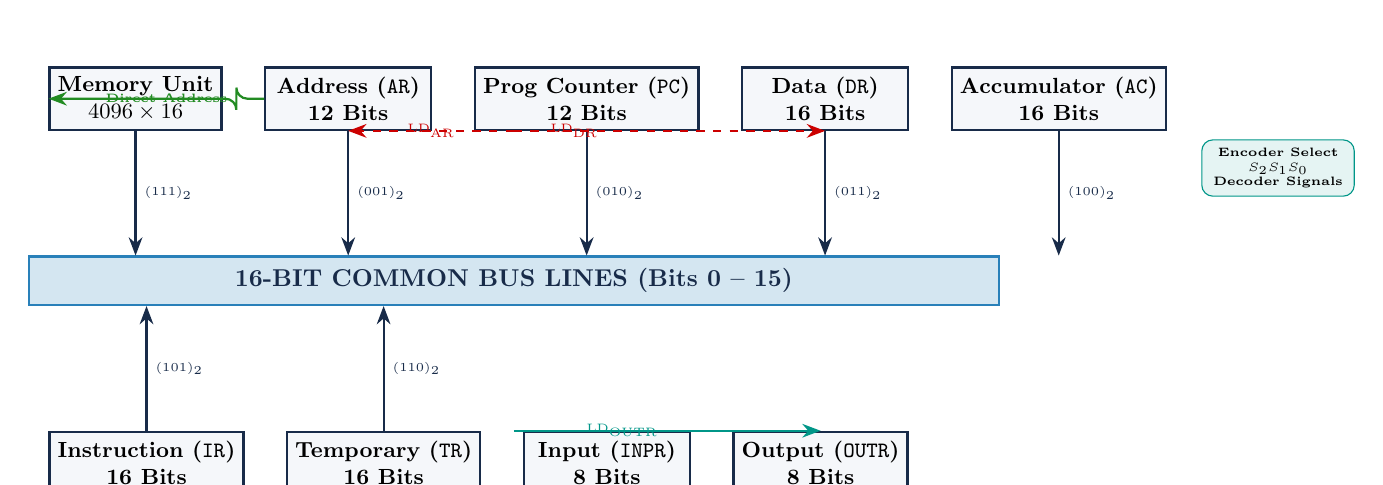
\begin{tikzpicture}[scale=0.88, transform shape,
    box/.style={rectangle, draw=primaryblue, fill=lightgrey, thick, minimum width=2.4cm, minimum height=0.9cm, align=center, font=\small\bfseries},
    bus/.style={rectangle, draw=secondaryblue, fill=secondaryblue!20, thick, minimum width=14cm, minimum height=0.7cm, align=center, font=\bfseries\color{primaryblue}},
    arrow/.style={-{Stealth[scale=1.0]}, thick, primaryblue},
    line/.style={thick, primaryblue}
]

% Common Bus Box
\node (BUS) [bus] {16-BIT COMMON BUS LINES (Bits 0 -- 15)};

% Registers Top Row
\node (MEMORY) [box, above=1.8cm of BUS.north west, anchor=south west, xshift=0.3cm] {Memory Unit\\$4096 \times 16$};
\node (AR)     [box, right=0.6cm of MEMORY] {Address (\texttt{AR})\\12 Bits};
\node (PC)     [box, right=0.6cm of AR]     {Prog Counter (\texttt{PC})\\12 Bits};
\node (DR)     [box, right=0.6cm of PC]     {Data (\texttt{DR})\\16 Bits};
\node (AC)     [box, right=0.6cm of DR]     {Accumulator (\texttt{AC})\\16 Bits};

% Registers Bottom Row
\node (IR)     [box, below=1.8cm of BUS.south west, anchor=north west, xshift=0.3cm] {Instruction (\texttt{IR})\\16 Bits};
\node (TR)     [box, right=0.6cm of IR]     {Temporary (\texttt{TR})\\16 Bits};
\node (INPR)   [box, right=0.6cm of TR]     {Input (\texttt{INPR})\\8 Bits};
\node (OUTR)   [box, right=0.6cm of INPR]   {Output (\texttt{OUTR})\\8 Bits};

% Arrows Top
\draw [arrow] (MEMORY.south) -- (MEMORY.south |- BUS.north) node[pos=0.5, right, font=\tiny] {$(111)_2$};
\draw [arrow] (AR.south) -- (AR.south |- BUS.north) node[pos=0.5, right, font=\tiny] {$(001)_2$};
\draw [arrow] (PC.south) -- (PC.south |- BUS.north) node[pos=0.5, right, font=\tiny] {$(010)_2$};
\draw [arrow] (DR.south) -- (DR.south |- BUS.north) node[pos=0.5, right, font=\tiny] {$(011)_2$};
\draw [arrow] (AC.south) -- (AC.south |- BUS.north) node[pos=0.5, right, font=\tiny] {$(100)_2$};

% Load Lines (Bus to Registers)
\draw [arrow, dashed, red!80!black] (BUS.north |- AR.south) -- (AR.south) node[pos=0.3, left, font=\tiny] {$\text{LD}_{\text{AR}}$};
\draw [arrow, dashed, red!80!black] (BUS.north |- DR.south) -- (DR.south) node[pos=0.3, left, font=\tiny] {$\text{LD}_{\text{DR}}$};

% Arrows Bottom
\draw [arrow] (IR.north) -- (IR.north |- BUS.south) node[pos=0.5, right, font=\tiny] {$(101)_2$};
\draw [arrow] (TR.north) -- (TR.north |- BUS.south) node[pos=0.5, right, font=\tiny] {$(110)_2$};
\draw [arrow, accentteal, thick] (BUS.south |- OUTR.north) -- (OUTR.north) node[pos=0.5, left, font=\tiny] {$\text{LD}_{\text{OUTR}}$};

% Direct Memory - AR Line
\draw [arrow, rounded corners, ForestGreen, thick] (AR.west) -- ++(-0.4,0) |- node[pos=0.25, left, font=\tiny\bfseries] {Direct Address} (MEMORY.west);

% Control Inputs Box
\node (CTRL) [rectangle, draw=accentteal, fill=accentteal!10, rounded corners, right=0.5cm of AC, yshift=-1.0cm, minimum width=2.2cm, font=\tiny\bfseries, align=center] {Encoder Select\\$S_2 S_1 S_0$\\Decoder Signals};

\end{tikzpicture}
\end{center}

\vspace{0.4cm}

\subsection{Instruction Fetch-Decode-Execute Cycle State Flow}

\begin{center}
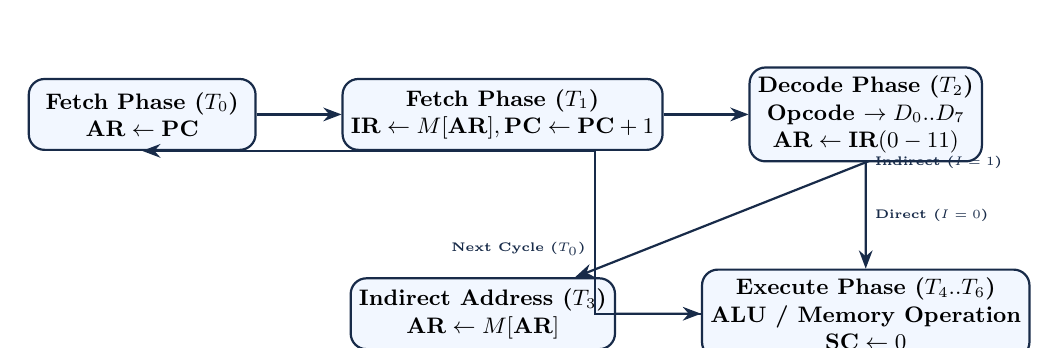
\begin{tikzpicture}[scale=0.9, transform shape,
    state/.style={rectangle, draw=primaryblue, fill=tablerowalt, rounded corners=2mm, thick, minimum width=3.2cm, minimum height=1.0cm, align=center, font=\small\bfseries},
    arrow/.style={-{Stealth[scale=1.0]}, thick, primaryblue}
]

\node (FETCH1)  [state] {Fetch Phase ($T_0$)\\$\text{AR} \leftarrow \text{PC}$};
\node (FETCH2)  [state, right=1.2cm of FETCH1] {Fetch Phase ($T_1$)\\$\text{IR} \leftarrow M[\text{AR}], \text{PC} \leftarrow \text{PC}+1$};
\node (DECODE)  [state, right=1.2cm of FETCH2] {Decode Phase ($T_2$)\\Opcode $\rightarrow D_0..D_7$\\$\text{AR} \leftarrow \text{IR}(0-11)$};
\node (EXEC)    [state, below=1.5cm of DECODE] {Execute Phase ($T_4..T_6$)\\ALU / Memory Operation\\$\text{SC} \leftarrow 0$};
\node (INDIRECT)[state, left=1.2cm of EXEC] {Indirect Address ($T_3$)\\$\text{AR} \leftarrow M[\text{AR}]$};

\draw [arrow] (FETCH1) -- (FETCH2);
\draw [arrow] (FETCH2) -- (DECODE);
\draw [arrow] (DECODE) -- node[right, font=\tiny\bfseries] {Indirect ($I=1$)} (EXEC |- DECODE.south) -- (INDIRECT);
\draw [arrow] (DECODE) -- node[right, font=\tiny\bfseries] {Direct ($I=0$)} (EXEC);
\draw [arrow] (INDIRECT) -- (EXEC);
\draw [arrow] (EXEC.west) -- ++(-1.5,0) |- node[pos=0.2, left, font=\tiny\bfseries] {Next Cycle ($T_0$)} (FETCH1.south);

\end{tikzpicture}
\end{center}

\vspace{0.4cm}

\subsection{ALU and Accumulator (\texttt{AC}) Microoperation Logic Block Diagram}

\begin{center}
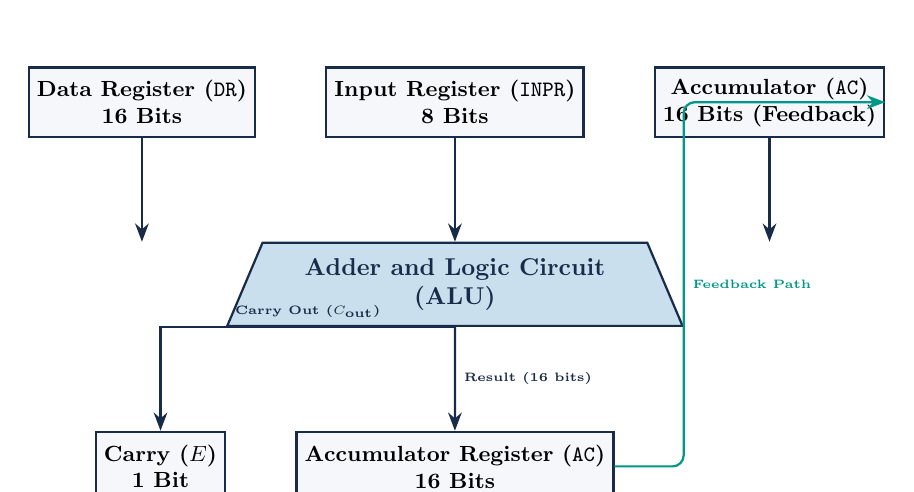
\begin{tikzpicture}[scale=0.88, transform shape,
    block/.style={rectangle, draw=primaryblue, fill=lightgrey, thick, minimum width=2.8cm, minimum height=1.0cm, align=center, font=\small\bfseries},
    alu/.style={trapezium, trapezium angle=67, draw=primaryblue, fill=secondaryblue!25, thick, minimum width=3.5cm, minimum height=1.2cm, align=center, font=\bfseries\color{primaryblue}},
    arrow/.style={-{Stealth[scale=1.0]}, thick, primaryblue}
]

\node (DR)   [block] {Data Register (\texttt{DR})\\16 Bits};
\node (INPR) [block, right=1.0cm of DR] {Input Register (\texttt{INPR})\\8 Bits};
\node (AC_IN)[block, right=1.0cm of INPR] {Accumulator (\texttt{AC})\\16 Bits (Feedback)};

\node (ALU)  [alu, below=1.5cm of INPR] {Adder and Logic Circuit\\(ALU)};

\node (AC_OUT)[block, below=1.5cm of ALU] {Accumulator Register (\texttt{AC})\\16 Bits};
\node (E_FF)  [block, left=1.0cm of AC_OUT, minimum width=1.5cm] {Carry ($E$)\\1 Bit};

\draw [arrow] (DR.south) -- (DR.south |- ALU.north);
\draw [arrow] (INPR.south) -- (INPR.south |- ALU.north);
\draw [arrow] (AC_IN.south) -- (AC_IN.south |- ALU.north);

\draw [arrow] (ALU.south) -- (AC_OUT.north) node[pos=0.5, right, font=\tiny\bfseries] {Result (16 bits)};
\draw [arrow] (ALU.south) -| (E_FF.north) node[pos=0.25, above, font=\tiny\bfseries] {Carry Out ($C_{\text{out}}$)};

\draw [arrow, rounded corners, accentteal, thick] (AC_OUT.east) -- ++(1.0,0) |- node[pos=0.25, right, font=\tiny\bfseries] {Feedback Path} (AC_IN.east);

\end{tikzpicture}
\end{center}

\vspace{0.4cm}

\begin{summarybox}{Conclusion}
The eight basic registers (\texttt{AR}, \texttt{PC}, \texttt{DR}, \texttt{AC}, \texttt{IR}, \texttt{TR}, \texttt{INPR}, \texttt{OUTR}) form the operational backbone of digital computer organization. Coupled with a 16-bit Common Bus system and timing signals generated by the Control Unit decoder, these registers orchestrate data movement, arithmetic computation, and input/output throughput with minimal hardware complexity.
\end{summarybox}

\end{document}
